\documentclass{standalone}
\usepackage{tikz}

\usetikzlibrary{circuits.logic.US,circuits.logic.IEC,circuits.ee.IEC}
\begin{document}
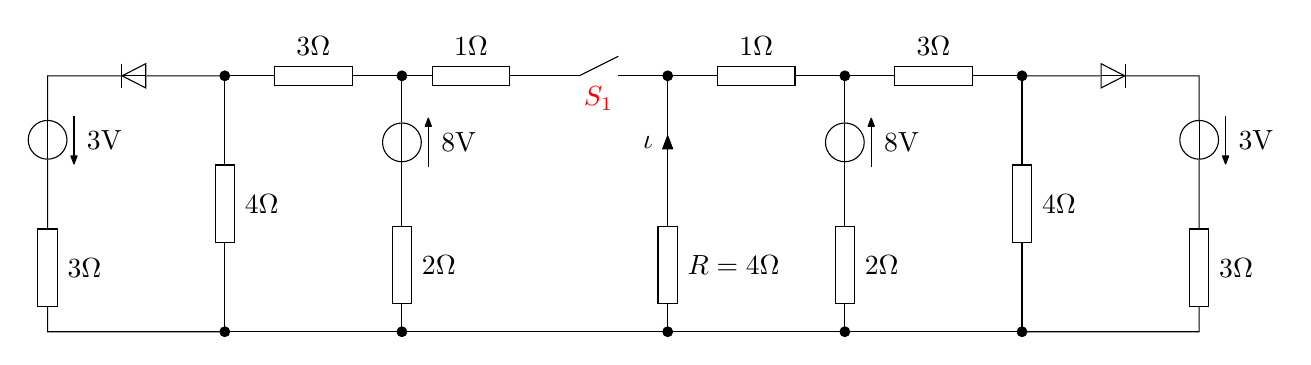
\begin{tikzpicture}[rotate=-90,circuit ee IEC,x=3.25cm,y=2.25cm]:
% Let us start with some contacts:
\foreach \contact/\y in {1/1,2/2,3/3.5,4/4.5,5/5.5}
{
\node [contact] (left contact \contact) at (0,\y) {};
\node [contact] (right contact \contact) at (1,\y) {};
}
\draw (right contact 1) -- (right contact 2) -- (right contact 3)
-- (right contact 4) -- (right contact 5);
\draw (left contact 1) to [diode] ++(down:1)
to [voltage source={near start,
direction info={volt=3}},
resistor={near end,ohm=3}] ++(right:1)
to (right contact 1);
\draw (left contact 1) to [resistor={ohm=4}] (right contact 1);
\draw (left contact 1) to [resistor={ohm=3}] (left contact 2);
\draw (left contact 2) to [voltage source={near start,
direction info={<-,volt=8}},
resistor={ohm=2,near end}] (right contact 2);
\draw (left contact 2) to [resistor={near start,ohm=1},
make contact={near end,info'={[red]$S_1$}}]
(left contact 3);
\draw (left contact 3) to [current direction'={near start,info=$\iota$},
resistor={near end,info={$R=4\Omega$}}]
(right contact 3);
\draw (left contact 4) to [voltage source={near start,
direction info={<-,volt=8}},
resistor={ohm=2,near end}] (right contact 4);
\draw (left contact 3) to [resistor={ohm=1}] (left contact 4);
\draw (left contact 4) to [resistor={ohm=3}] (left contact 5);
\draw (left contact 5) to [resistor={ohm=4}] (right contact 5);
\draw (left contact 5) to [diode] ++(up:1)
to [voltage source={near start,
direction info={volt=3}},
resistor={near end,ohm=3}] ++(right:1)
to (right contact 5);
\end{tikzpicture}
\end{document}